\documentclass{article}

% content/resources/templates/preamble.tex
\usepackage[margin=0.6in]{geometry}
\author{Milav Dabgar}
\usepackage{amsmath,amssymb,amsthm}
\usepackage{booktabs}
\usepackage{multirow}
\usepackage{xcolor}
\usepackage{tcolorbox}
\tcbuselibrary{breakable,skins}
\usepackage[colorlinks=true,linkcolor=blue]{hyperref}
\usepackage{titlesec}
\usepackage{enumitem}
\usepackage{tikz}
\usepackage{pgfplots}
\usepackage{circuitikz}
\usepackage[version=4]{mhchem}
\usepackage{longtable}
\usepackage{array}
\usepackage{float}
\usepackage{caption}
\usepackage{listings}

\lstset{
  basicstyle=\small\ttfamily,
  breaklines=true,
  breakatwhitespace=false,
  postbreak=\mbox{\textcolor{red}{$\hookrightarrow$}\space},
  float=false,
  numbers=left,
  numberstyle=\tiny\color{gray},
  numbersep=10pt,
  xleftmargin=2em,
  keywordstyle=\color{blue},
  commentstyle=\color{green!60!black},
  stringstyle=\color{purple},
  backgroundcolor=\color{gray!5},
  showstringspaces=false,
  tabsize=2,
  captionpos=b,
  keepspaces=true,
  columns=flexible
}

\pgfplotsset{compat=1.18}
\usetikzlibrary{shapes,arrows,positioning,calc,patterns,decorations.pathmorphing,decorations.markings,arrows.meta}

% Color scheme
\definecolor{headcolor}{RGB}{0,102,204}
\definecolor{keycolor}{RGB}{220,20,60}
\definecolor{solutioncolor}{RGB}{34,139,34}
\definecolor{mnemoniccolor}{RGB}{148,0,211}
\definecolor{codecolor}{RGB}{0,0,100}

% Spacing
\setlength{\parskip}{3pt}
\setlist[itemize]{nosep}
\setlist[enumerate]{nosep}

% Title formatting
\titleformat{\section}{\Large\bfseries\color{headcolor}}{\thesection}{1em}{}
\titleformat{\subsection}{\large\bfseries\color{headcolor}}{\thesubsection}{1em}{}

% Pandoc tightlist compatibility
\providecommand{\tightlist}{%
  \setlength{\itemsep}{0pt}\setlength{\parskip}{0pt}}

% Pandoc longtable compatibility
\newcounter{none}
\def\thenone{}


% content/resources/templates/english-boxes.tex

% Custom environments
\newtcolorbox{solutionbox}{
 breakable,
 enhanced,
 colback=solutioncolor!5!white,
 colframe=solutioncolor!75!black,
 fonttitle=\bfseries,
 title=Solution
}

\newtcolorbox{solutionboxnobreak}{
 colback=solutioncolor!5!white,
 colframe=solutioncolor!75!black,
 fonttitle=\bfseries,
 title=Solution
}

\newtcolorbox{keyformula}{
 breakable,
 enhanced,
 colback=keycolor!5!white,
 colframe=keycolor!75!black,
 fonttitle=\bfseries,
 title=Key Formula
}

\newtcolorbox{mnemonicboxenv}{
 breakable,
 enhanced,
 colback=mnemoniccolor!5!white,
 colframe=mnemoniccolor!75!black,
 fonttitle=\bfseries,
 title=Mnemonic
}

\newcommand{\mnemonicbox}[1]{%
  \begin{mnemonicboxenv}
    #1
  \end{mnemonicboxenv}
}


% Custom commands for GTU solutions
% This file defines semantic commands for consistent formatting

% Question command with automatic formatting
\newcommand{\question}[2]{%
  \section*{Question #1}%
  \textbf{#2}%
}

% OR question variant
\newcommand{\questionor}[2]{%
  \section*{Question #1 OR}%
  \textbf{#2}%
}

% Proper table environment with caption
\newenvironment{answertable}[1]{%
  \begin{table}[htbp]
  \centering
  \caption{#1}
}{%
  \end{table}
}

% Proper figure environment for diagrams
\newenvironment{answerdiagram}[1]{%
  \begin{figure}[htbp]
  \centering
  \caption{#1}
}{%
  \end{figure}
}

% Semantic markup for key terms
\newcommand{\keyword}[1]{\textbf{#1}}
\newcommand{\code}[1]{\texttt{#1}}
\newcommand{\classname}[1]{\texttt{#1}}
\newcommand{\methodname}[1]{\texttt{#1}}

% Proper quotation marks
\newcommand{\mnemonic}[1]{``#1''}


\title{Foundation of Blockchain (4361603) - Winter 2024 Solution}
\date{November 25, 2024}

\begin{document}
\maketitle

\questionmarks{1(a)}{3}{Short Note on: Distributed Ledger}

\begin{solutionbox}
\textbf{Answer}:

\begin{center}
\captionof{table}{Distributed Ledger Features}
\begin{tabulary}{\linewidth}{L L}
    \toprule
    \textbf{Feature} & \textbf{Description} \\
    \midrule
    \textbf{Definition} & Database spread across multiple computers \\
    \textbf{Storage} & Data stored in multiple locations \\
    \textbf{Control} & No single authority owns it \\
    \textbf{Updates} & All copies updated simultaneously \\
    \bottomrule
\end{tabulary}
\end{center}

\begin{itemize}
    \item \keyword{Decentralized}: No central server needed
    \item \keyword{Transparent}: All participants can see transactions
    \item \keyword{Secure}: Uses cryptography for protection
\end{itemize}
\end{solutionbox}

\begin{mnemonicbox}
Data Stored Transparently Securely (DSTS)
\end{mnemonicbox}

\questionmarks{1(b)}{4}{Describe the applications of Blockchain.}

\begin{solutionbox}
\textbf{Answer}:

\begin{center}
\captionof{table}{Blockchain Applications}
\begin{tabulary}{\linewidth}{L L L}
    \toprule
    \textbf{Application} & \textbf{Use Case} & \textbf{Benefit} \\
    \midrule
    \textbf{Cryptocurrency} & Digital money like Bitcoin & Secure payments \\
    \textbf{Supply Chain} & Track products from source & Prevent fake goods \\
    \textbf{Healthcare} & Store medical records & Data security \\
    \textbf{Voting} & Electronic voting system & Transparent elections \\
    \textbf{Real Estate} & Property records & Fraud prevention \\
    \bottomrule
\end{tabulary}
\end{center}

\begin{itemize}
    \item \keyword{Finance}: Faster cross-border payments
    \item \keyword{Identity}: Digital ID verification
    \item \keyword{Smart Contracts}: Automated agreements
\end{itemize}
\end{solutionbox}

\begin{mnemonicbox}
Money, Medicine, Voting, Property (MMVP)
\end{mnemonicbox}

\questionmarks{1(c)}{7}{Explain Asymmetric Encryption Model with example.}

\begin{solutionbox}
\textbf{Answer}:

\textbf{Asymmetric Encryption Process}

\begin{center}
    \begin{tikzpicture}[node distance=1.5cm, auto]
        \node [gtu state] (Sender) {Sender};
        \node [gtu block, right=of Sender] (PubKey) {Public Key};
        \node [gtu block, right=of PubKey] (Encrypt) {Encrypt Message};
        \node [gtu block, below=of Encrypt] (Data) {Encrypted Data};
        \node [gtu block, left=of Data] (Receiver) {Receiver};
        \node [gtu block, left=of Receiver] (PrivKey) {Private Key};
        \node [gtu block, below=of PrivKey] (Decrypt) {Decrypt Message};
        \node [gtu state, right=of Decrypt] (Msg) {Original Message};

        \draw [gtu arrow] (Sender) -- (PubKey);
        \draw [gtu arrow] (PubKey) -- (Encrypt);
        \draw [gtu arrow] (Encrypt) -- (Data);
        \draw [gtu arrow] (Data) -- (Receiver);
        \draw [gtu arrow] (Receiver) -- (PrivKey);
        \draw [gtu arrow] (PrivKey) -- (Decrypt);
        \draw [gtu arrow] (Decrypt) -- (Msg);
    \end{tikzpicture}
    \captionof{figure}{Asymmetric Encryption Workflow}
\end{center}

\begin{center}
\captionof{table}{Key Comparison}
\begin{tabulary}{\linewidth}{L L L L}
    \toprule
    \textbf{Key Type} & \textbf{Purpose} & \textbf{Sharing} & \textbf{Example} \\
    \midrule
    \textbf{Public Key} & Encryption & Shared openly & RSA Public Key \\
    \textbf{Private Key} & Decryption & Kept secret & RSA Private Key \\
    \bottomrule
\end{tabulary}
\end{center}

\textbf{Example Process:}

\begin{enumerate}
    \item Alice wants to send message to Bob
    \item Alice uses Bob's public key to encrypt
    \item Only Bob's private key can decrypt
    \item Bob receives and decrypts message
\end{enumerate}

\begin{itemize}
    \item \keyword{Security}: Even if public key is known, data stays safe
    \item \keyword{Authentication}: Proves sender identity
    \item \keyword{Non-repudiation}: Sender cannot deny sending
\end{itemize}
\end{solutionbox}

\begin{mnemonicbox}
Public Encrypts, Private Decrypts (PEPD)
\end{mnemonicbox}

\orquestionmarks{1(c)}{7}{Explain Consistency, Availability and Partition Tolerance (CAP) theorem in Blockchain.}

\begin{solutionbox}
\textbf{Answer}:

\textbf{CAP Theorem Triangle}

\begin{center}
    \begin{tikzpicture}[node distance=2.5cm, auto]
        \node [gtu state] (C) {Consistency};
        \node [gtu state, below left=of C] (A) {Availability};
        \node [gtu state, below right=of C] (P) {Partition Tolerance};
        
        \path (C) -- node[midway] (CA) {} (A);
        \path (A) -- node[midway] (AP) {} (P);
        \path (P) -- node[midway] (PC) {} (C);
        
        \node [gtu block, align=center] at (barycentric cs:C=1,A=1,P=1) {CAP Theorem};
        
        \node [below=0.2cm of C, font=\footnotesize] {All nodes see same data};
        \node [below=0.2cm of A, font=\footnotesize] {System always responds};
        \node [below=0.2cm of P, font=\footnotesize] {Works despite failures};

        \draw [gtu arrow, <->] (C) -- (A);
        \draw [gtu arrow, <->] (A) -- (P);
        \draw [gtu arrow, <->] (P) -- (C);
    \end{tikzpicture}
    \captionof{figure}{CAP Theorem Properties}
\end{center}

\begin{center}
\captionof{table}{CAP Properties}
\begin{tabulary}{\linewidth}{L L L}
    \toprule
    \textbf{Property} & \textbf{Definition} & \textbf{Blockchain Focus} \\
    \midrule
    \textbf{Consistency} & All nodes have same data & Medium priority \\
    \textbf{Availability} & System always responds & High priority \\
    \textbf{Partition Tolerance} & Works with network splits & High priority \\
    \bottomrule
\end{tabulary}
\end{center}

\textbf{Key Points:}

\begin{itemize}
    \item \keyword{Trade-off}: Can only guarantee 2 out of 3 properties
    \item \keyword{Blockchain Choice}: Usually prioritizes Availability + Partition Tolerance
    \item \keyword{Real Example}: Bitcoin chooses AP over C (eventual consistency)
\end{itemize}
\end{solutionbox}

\begin{mnemonicbox}
Choose Any Two (CAT)
\end{mnemonicbox}

\questionmarks{2(a)}{3}{Define: Public key, Private key, Digital Signature.}

\begin{solutionbox}
\textbf{Answer}:

\begin{center}
\captionof{table}{Cryptographic Components}
\begin{tabulary}{\linewidth}{L L L}
    \toprule
    \textbf{Component} & \textbf{Definition} & \textbf{Usage} \\
    \midrule
    \textbf{Public Key} & Encryption key shared openly & Encrypt data, verify signatures \\
    \textbf{Private Key} & Secret key kept by owner & Decrypt data, create signatures \\
    \textbf{Digital Signature} & Encrypted hash of message & Prove authenticity and integrity \\
    \bottomrule
\end{tabulary}
\end{center}
\end{solutionbox}

\begin{mnemonicbox}
Public Protects, Private Proves (PPPP)
\end{mnemonicbox}

\questionmarks{2(b)}{4}{Explain Public blockchain with its advantage and disadvantage.}

\begin{solutionbox}
\textbf{Answer}:

\begin{center}
\captionof{table}{Public Blockchain Analysis}
\begin{tabulary}{\linewidth}{L L}
    \toprule
    \textbf{Aspect} & \textbf{Details} \\
    \midrule
    \textbf{Definition} & Open network accessible to everyone \\
    \textbf{Examples} & Bitcoin, Ethereum \\
    \bottomrule
\end{tabulary}
\end{center}

\textbf{Advantages:}

\begin{itemize}
    \item \keyword{Transparency}: All transactions visible
    \item \keyword{Decentralization}: No single control
    \item \keyword{Security}: Many nodes validate
\end{itemize}

\textbf{Disadvantages:}

\begin{itemize}
    \item \keyword{Speed}: Slow transaction processing
    \item \keyword{Energy}: High power consumption
    \item \keyword{Scalability}: Limited transactions per second
\end{itemize}
\end{solutionbox}

\begin{mnemonicbox}
Transparent but Slow (TBS)
\end{mnemonicbox}

\questionmarks{2(c)}{7}{Describe Core components of Blockchain.}

\begin{solutionbox}
\textbf{Answer}:

\textbf{Blockchain Structure}

\begin{center}
    \begin{tikzpicture}[node distance=1.5cm, auto]
        \node [gtu block] (BN) {Block N};
        \node [gtu block, left=of BN] (BNm1) {Block N-1};
        \node [gtu block, right=of BN] (BNp1) {Block N+1};
        
        \node [gtu block, below=of BN, align=center] (Details) {Block Header\\Transactions};
        
        \node [gtu interval, below=of Details, align=center] (Components) {Previous Hash\\Merkle Root\\Timestamp\\Nonce};
        
        \draw [gtu arrow] (BNm1) -- (BN);
        \draw [gtu arrow] (BN) -- (BNp1);
        \draw [gtu arrow] (BN) -- (Details);
        \draw [gtu arrow] (Details) -- (Components);
    \end{tikzpicture}
    \captionof{figure}{Core Blockchain Components}
\end{center}

\begin{center}
\captionof{table}{Core Components}
\begin{tabulary}{\linewidth}{L L L}
    \toprule
    \textbf{Component} & \textbf{Function} & \textbf{Importance} \\
    \midrule
    \textbf{Block} & Container for transactions & Data storage \\
    \textbf{Hash} & Unique identifier & Security \\
    \textbf{Merkle Tree} & Transaction summary & Verification \\
    \textbf{Nonce} & Mining number & Proof of work \\
    \textbf{Timestamp} & Time record & Chronological order \\
    \textbf{Previous Hash} & Links to previous block & Chain integrity \\
    \bottomrule
\end{tabulary}
\end{center}

\begin{itemize}
    \item \keyword{Immutability}: Cannot change past records
    \item \keyword{Transparency}: All data visible
    \item \keyword{Consensus}: Network agrees on validity
\end{itemize}
\end{solutionbox}

\begin{mnemonicbox}
Blocks Hash Merkle Nonce Time Previous (BHMNTP)
\end{mnemonicbox}

\orquestionmarks{2(a)}{3}{Short Note on: SideChain}

\begin{solutionbox}
\textbf{Answer}:

\begin{center}
\captionof{table}{SideChain Features}
\begin{tabulary}{\linewidth}{L L}
    \toprule
    \textbf{Feature} & \textbf{Description} \\
    \midrule
    \textbf{Definition} & Separate blockchain connected to main chain \\
    \textbf{Purpose} & Extend main blockchain functionality \\
    \textbf{Connection} & Two-way peg mechanism \\
    \bottomrule
\end{tabulary}
\end{center}

\begin{itemize}
    \item \keyword{Scalability}: Reduces main chain load
    \item \keyword{Flexibility}: Custom features possible
    \item \keyword{Security}: Inherits main chain security
\end{itemize}
\end{solutionbox}

\begin{mnemonicbox}
Separate Side Scales (SSS)
\end{mnemonicbox}

\orquestionmarks{2(b)}{4}{Explain Private blockchain with its advantage and disadvantage.}

\begin{solutionbox}
\textbf{Answer}:

\begin{center}
\captionof{table}{Private Blockchain Analysis}
\begin{tabulary}{\linewidth}{L L}
    \toprule
    \textbf{Aspect} & \textbf{Details} \\
    \midrule
    \textbf{Definition} & Restricted network with controlled access \\
    \textbf{Control} & Single organization manages \\
    \bottomrule
\end{tabulary}
\end{center}

\textbf{Advantages:}

\begin{itemize}
    \item \keyword{Speed}: Faster transactions
    \item \keyword{Privacy}: Controlled data access
    \item \keyword{Efficiency}: Lower energy consumption
    \item \keyword{Compliance}: Meets regulatory requirements
\end{itemize}

\textbf{Disadvantages:}

\begin{itemize}
    \item \keyword{Centralization}: Single point of control
    \item \keyword{Trust}: Relies on controlling organization
    \item \keyword{Limited}: Fewer participants
\end{itemize}
\end{solutionbox}

\begin{mnemonicbox}
Fast Private Controlled (FPC)
\end{mnemonicbox}

\orquestionmarks{2(c)}{7}{Explain Data structure of Blockchain.}

\begin{solutionbox}
\textbf{Answer}:

\textbf{Blockchain Data Structure}

\begin{center}
    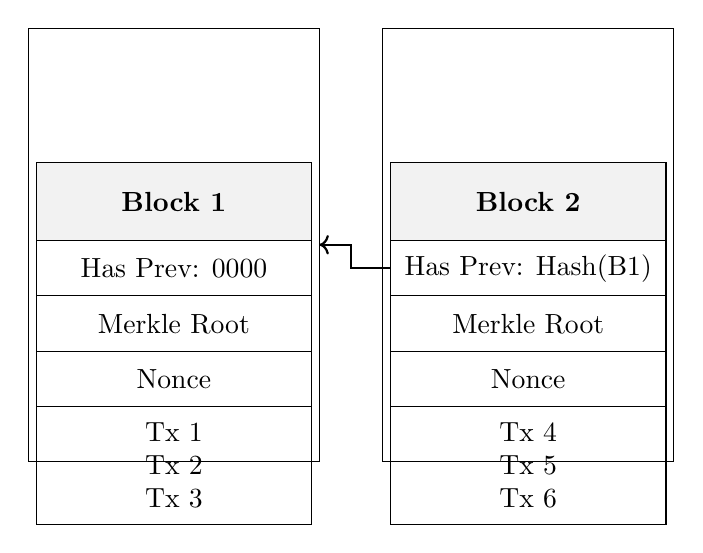
\begin{tikzpicture}[node distance=0cm, outer sep=0pt]
        % Block 1
        \node [draw, rectangle, minimum width=3.5cm, minimum height=1cm, fill=gray!10] (Head1) {\textbf{Block 1}};
        \node [draw, rectangle, minimum width=3.5cm, minimum height=0.7cm, below=0pt of Head1] (Prev1) {Has Prev: 0000};
        \node [draw, rectangle, minimum width=3.5cm, minimum height=0.7cm, below=0pt of Prev1] (Merkle1) {Merkle Root};
        \node [draw, rectangle, minimum width=3.5cm, minimum height=0.7cm, below=0pt of Merkle1] (Nonce1) {Nonce};
        \node [draw, rectangle, minimum width=3.5cm, minimum height=1.5cm, below=0pt of Nonce1, align=center] (Tx1) {Tx 1\\Tx 2\\Tx 3};
        
        \node [draw, rectangle, minimum width=3.7cm, minimum height=5.5cm, below=0pt of Head1, yshift=2.7cm] (Block1) {};

        % Block 2
        \node [draw, rectangle, minimum width=3.5cm, minimum height=1cm, fill=gray!10, right=1cm of Head1] (Head2) {\textbf{Block 2}};
        \node [draw, rectangle, minimum width=3.5cm, minimum height=0.7cm, below=0pt of Head2] (Prev2) {Has Prev: Hash(B1)};
        \node [draw, rectangle, minimum width=3.5cm, minimum height=0.7cm, below=0pt of Prev2] (Merkle2) {Merkle Root};
        \node [draw, rectangle, minimum width=3.5cm, minimum height=0.7cm, below=0pt of Merkle2] (Nonce2) {Nonce};
        \node [draw, rectangle, minimum width=3.5cm, minimum height=1.5cm, below=0pt of Nonce2, align=center] (Tx2) {Tx 4\\Tx 5\\Tx 6};
        
        \node [draw, rectangle, minimum width=3.7cm, minimum height=5.5cm, below=0pt of Head2, yshift=2.7cm] (Block2) {};

        % Arrows
        \draw [thick, ->] (Prev2.west) -- ++(-0.5,0) |- (Block1.east);
    \end{tikzpicture}
    \captionof{figure}{Blockchain Linked List Structure}
\end{center}

\begin{center}
\captionof{table}{Data Structure Elements}
\begin{tabulary}{\linewidth}{L L L}
    \toprule
    \textbf{Element} & \textbf{Purpose} & \textbf{Size} \\
    \midrule
    \textbf{Block Header} & Contains metadata & Fixed size \\
    \textbf{Transaction List} & Actual data & Variable size \\
    \textbf{Hash Pointer} & Links blocks & 256 bits \\
    \textbf{Merkle Tree} & Transaction summary & Logarithmic \\
    \bottomrule
\end{tabulary}
\end{center}

\textbf{Key Features:}

\begin{itemize}
    \item \keyword{Linear Structure}: Blocks linked in sequence
    \item \keyword{Hash Linking}: Each block references previous
    \item \keyword{Merkle Trees}: Efficient transaction verification
    \item \keyword{Immutable}: Cannot modify without detection
\end{itemize}
\end{solutionbox}

\begin{mnemonicbox}
Linear Hash Merkle Immutable (LHMI)
\end{mnemonicbox}

\questionmarks{3(a)}{3}{Short Note on: Consensus Mechanism in Blockchain.}

\begin{solutionbox}
\textbf{Answer}:

\begin{center}
\captionof{table}{Consensus Mechanism}
\begin{tabulary}{\linewidth}{L L}
    \toprule
    \textbf{Aspect} & \textbf{Description} \\
    \midrule
    \textbf{Purpose} & Agree on network state \\
    \textbf{Need} & Prevent double spending \\
    \textbf{Types} & PoW, PoS, DPoS \\
    \bottomrule
\end{tabulary}
\end{center}

\begin{itemize}
    \item \keyword{Agreement}: All nodes must agree
    \item \keyword{Decentralization}: No central authority
    \item \keyword{Security}: Prevents malicious activities
\end{itemize}
\end{solutionbox}

\begin{mnemonicbox}
Agreement Prevents Security (APS)
\end{mnemonicbox}

\questionmarks{3(b)}{4}{Compare Hard Fork and Soft Fork in Blockchain.}

\begin{solutionbox}
\textbf{Answer}:

\begin{center}
\captionof{table}{Fork Comparison}
\begin{tabulary}{\linewidth}{L L L}
    \toprule
    \textbf{Feature} & \textbf{Hard Fork} & \textbf{Soft Fork} \\
    \midrule
    \textbf{Compatibility} & Not backward compatible & Backward compatible \\
    \textbf{Rules} & Creates new rules & Tightens existing rules \\
    \textbf{Upgrade} & All nodes must upgrade & Optional upgrade \\
    \textbf{Result} & Two separate chains & Single chain continues \\
    \textbf{Example} & Ethereum to Ethereum Classic & Bitcoin SegWit \\
    \bottomrule
\end{tabulary}
\end{center}

\textbf{Key Differences:}

\begin{itemize}
    \item \keyword{Hard Fork}: Permanent split in blockchain
    \item \keyword{Soft Fork}: Temporary restriction that becomes permanent
\end{itemize}
\end{solutionbox}

\begin{mnemonicbox}
Hard Splits, Soft Restricts (HSSR)
\end{mnemonicbox}

\questionmarks{3(c)}{7}{What is Proof of Work? How does it work? Explain with example.}

\begin{solutionbox}
\textbf{Answer}:

\textbf{Proof of Work Process}

\begin{center}
    \begin{tikzpicture}[node distance=1.5cm, auto]
        \node [gtu state] (New) {New Transactions};
        \node [gtu block, right=of New] (Create) {Create Block};
        \node [gtu block, right=of Create] (Hash) {Calculate Hash};
        \node [draw, diamond, aspect=2, below=of Hash] (Check) {Hash < Target?};
        
        \node [gtu block, left=of Check] (Change) {Change Nonce};
        \node [gtu block, right=of Check] (Valid) {Block Valid};
        \node [gtu block, below=of Valid] (Add) {Add to Blockchain};
        
        \draw [gtu arrow] (New) -- (Create);
        \draw [gtu arrow] (Create) -- (Hash);
        \draw [gtu arrow] (Hash) -- (Check);
        \draw [gtu arrow] (Check) -- node[above] {Yes} (Valid);
        \draw [gtu arrow] (Check.west) -- node[above] {No} (Change);
        \draw [gtu arrow] (Change.north) |- (Hash.west);
        \draw [gtu arrow] (Valid) -- (Add);
    \end{tikzpicture}
    \captionof{figure}{Mining and PoW Workflow}
\end{center}

\begin{center}
\captionof{table}{PoW Components}
\begin{tabulary}{\linewidth}{L L L}
    \toprule
    \textbf{Component} & \textbf{Function} & \textbf{Example} \\
    \midrule
    \textbf{Hash Function} & Creates unique fingerprint & SHA-256 \\
    \textbf{Nonce} & Random number to change hash & 12345 \\
    \textbf{Difficulty} & Required number of leading zeros & 4 zeros \\
    \textbf{Mining} & Computing process & Bitcoin mining \\
    \bottomrule
\end{tabulary}
\end{center}

\textbf{Working Process:}

\begin{enumerate}
    \item Collect pending transactions
    \item Create block with transactions
    \item Try different nonce values
    \item Calculate hash repeatedly
    \item Find hash with required zeros
    \item Broadcast valid block to network
\end{enumerate}

\textbf{Bitcoin Example:}

\begin{itemize}
    \item \keyword{Target}: Hash must start with specific zeros
    \item \keyword{Time}: ~10 minutes per block
    \item \keyword{Reward}: 6.25 BTC (as of 2024)
\end{itemize}
\end{solutionbox}

\begin{mnemonicbox}
Try Calculate Until Zero (TCUZ)
\end{mnemonicbox}

\orquestionmarks{3(a)}{3}{Short Note on: Block Rewards in Blockchain.}

\begin{solutionbox}
\textbf{Answer}:

\begin{center}
\captionof{table}{Block Rewards Analysis}
\begin{tabulary}{\linewidth}{L L}
    \toprule
    \textbf{Feature} & \textbf{Description} \\
    \midrule
    \textbf{Purpose} & Incentivize miners \\
    \textbf{Components} & Block reward + transaction fees \\
    \textbf{Bitcoin} & Started at 50 BTC, halves every 4 years \\
    \bottomrule
\end{tabulary}
\end{center}

\begin{itemize}
    \item \keyword{Motivation}: Encourages network participation
    \item \keyword{Halving}: Reduces inflation over time
    \item \keyword{Fees}: Additional income for miners
\end{itemize}
\end{solutionbox}

\begin{mnemonicbox}
Miners Motivated Money (MMM)
\end{mnemonicbox}

\orquestionmarks{3(b)}{4}{What is 51\% attack and how does it work?}

\begin{solutionbox}
\textbf{Answer}:

\begin{center}
\captionof{table}{51\% Attack Analysis}
\begin{tabulary}{\linewidth}{L L}
    \toprule
    \textbf{Aspect} & \textbf{Details} \\
    \midrule
    \textbf{Definition} & Controlling majority mining power \\
    \textbf{Threshold} & More than 50\% network hash rate \\
    \textbf{Capability} & Can reverse transactions \\
    \textbf{Limitation} & Cannot steal others' coins \\
    \bottomrule
\end{tabulary}
\end{center}

\textbf{How it Works:}

\begin{enumerate}
    \item Attacker gains majority mining power
    \item Creates private blockchain fork
    \item Mines faster than honest network
    \item Releases longer chain to network
    \item Network accepts longer chain as valid
\end{enumerate}

\begin{center}
    \begin{tikzpicture}[node distance=1.5cm]
        \node [gtu block] (B_N) {Block N};
        
        % Honest Chain
        \node [gtu block, above right=1cm and 2cm of B_N] (Honest1) {Block N+1};
        \node [right=0.2cm of Honest1] {Honest Chain (Abandoned)};
        
        % Attacker Chain
        \node [gtu block, below right=1cm and 2cm of B_N, fill=red!10] (Bad1) {Block N'+1};
        \node [gtu block, right=of Bad1, fill=red!10] (Bad2) {Block N'+2 (Longer)};
        \node [right=0.2cm of Bad2] {Attacker Chain (Accepted)};

        \draw [gtu arrow] (B_N) -- (Honest1);
        \draw [gtu arrow] (B_N) -- (Bad1);
        \draw [gtu arrow] (Bad1) -- (Bad2);
    \end{tikzpicture}
    \captionof{figure}{51\% Attack Mechanism}
\end{center}

\begin{itemize}
    \item \keyword{Double Spending}: Spend same coins twice
    \item \keyword{Transaction Reversal}: Cancel confirmed transactions
\end{itemize}
\end{solutionbox}

\begin{mnemonicbox}
Majority Controls Chain (MCC)
\end{mnemonicbox}

\orquestionmarks{3(c)}{7}{What is Proof of Stake? How does it work? Explain with example.}

\begin{solutionbox}
\textbf{Answer}:

\textbf{Proof of Stake Process}

\begin{center}
    \begin{tikzpicture}[node distance=1.5cm, auto]
        \node [gtu state] (Stake) {Validators Stake Coins};
        \node [gtu block, right=of Stake] (Select) {Random Selection};
        \node [gtu block, right=of Select] (Prop) {Propose Block};
        \node [gtu block, below=of Prop] (Vote) {Validators Vote};
        \node [draw, diamond, aspect=2, below=of Vote] (Cons) {Consensus?};
        
        \node [gtu block, left=of Cons] (Add) {Block Added};
        \node [gtu state, below=of Add] (Reward) {Reward};
        \node [gtu state, right=of Cons] (Slash) {Penalty};
        
        \draw [gtu arrow] (Stake) -- (Select);
        \draw [gtu arrow] (Select) -- (Prop);
        \draw [gtu arrow] (Prop) -- (Vote);
        \draw [gtu arrow] (Vote) -- (Cons);
        \draw [gtu arrow] (Cons) -- node[above] {Yes} (Add);
        \draw [gtu arrow] (Add) -- (Reward);
        \draw [gtu arrow] (Cons) -- node[above] {No} (Slash);
    \end{tikzpicture}
    \captionof{figure}{Proof of Stake Workflow}
\end{center}

\textbf{PoS vs PoW}

\begin{center}
\captionof{table}{PoS vs PoW}
\begin{tabulary}{\linewidth}{L L L}
    \toprule
    \textbf{Feature} & \textbf{Proof of Stake} & \textbf{Proof of Work} \\
    \midrule
    \textbf{Energy} & Low consumption & High consumption \\
    \textbf{Selection} & Stake-based & Computing power \\
    \textbf{Hardware} & Regular computer & Specialized miners \\
    \textbf{Speed} & Faster & Slower \\
    \bottomrule
\end{tabulary}
\end{center}

\textbf{Ethereum Example:}

\begin{itemize}
    \item \keyword{Minimum Stake}: 32 ETH required
    \item \keyword{Penalties}: Slashing for malicious behavior
    \item \keyword{Benefits}: Energy efficient and scalable
\end{itemize}
\end{solutionbox}

\begin{mnemonicbox}
Stake Select Validate Reward (SSVR)
\end{mnemonicbox}

\questionmarks{4(a)}{3}{Describe Byzantine Fault Tolerance.}

\begin{solutionbox}
\textbf{Answer}:

\begin{center}
\captionof{table}{Byzantine Fault Tolerance Key Aspects}
\begin{tabulary}{\linewidth}{L L}
    \toprule
    \textbf{Aspect} & \textbf{Description} \\
    \midrule
    \textbf{Problem} & Some nodes may act maliciously \\
    \textbf{Tolerance} & System works despite faulty nodes \\
    \textbf{Requirement} & Less than 1/3 nodes can be faulty \\
    \bottomrule
\end{tabulary}
\end{center}

\begin{itemize}
    \item \keyword{Consensus}: Honest nodes must agree
    \item \keyword{Resilience}: Network survives attacks
\end{itemize}
\end{solutionbox}

\begin{mnemonicbox}
Faulty Nodes Tolerated (FNT)
\end{mnemonicbox}

\questionmarks{4(b)}{4}{How smart contract works in blockchain?}

\begin{solutionbox}
\textbf{Answer}:

\textbf{Smart Contract Execution}

\begin{center}
    \begin{tikzpicture}[node distance=1.5cm, auto]
        \node [gtu block] (Create) {Contract Created};
        \node [gtu block, right=of Create] (Deploy) {Deployed on Blockchain};
        \node [gtu block, below=of Deploy] (Cond) {Conditions Met};
        \node [gtu state, left=of Cond] (Exec) {Automatic Execution};
        \node [gtu state, left=of Exec] (Rec) {Results Recorded};
        
        \draw [gtu arrow] (Create) -- (Deploy);
        \draw [gtu arrow] (Deploy) -- (Cond);
        \draw [gtu arrow] (Cond) -- (Exec);
        \draw [gtu arrow] (Exec) -- (Rec);
    \end{tikzpicture}
    \captionof{figure}{Smart Contract Lifecycle}
\end{center}

\textbf{Working Process:}

\begin{enumerate}
    \item \textbf{Creation}: Developer writes contract code
    \item \textbf{Deployment}: Contract stored on blockchain
    \item \textbf{Trigger}: External event activates contract
    \item \textbf{Execution}: Code runs automatically
\end{enumerate}
\end{solutionbox}

\begin{mnemonicbox}
Code Executes Automatically (CEA)
\end{mnemonicbox}

\questionmarks{4(c)}{7}{What is SHA-256 and what is the use of SHA-256 in Blockchain.}

\begin{solutionbox}
\textbf{Answer}:

\begin{center}
\captionof{table}{SHA-256 Properties}
\begin{tabulary}{\linewidth}{L L}
    \toprule
    \textbf{Property} & \textbf{Description} \\
    \midrule
    \textbf{Full Name} & Secure Hash Algorithm 256-bit \\
    \textbf{Output} & Always 256 bits (64 hex characters) \\
    \textbf{Input} & Any size data \\
    \textbf{Nature} & One-way function \\
    \bottomrule
\end{tabulary}
\end{center}

\textbf{SHA-256 in Blockchain}

\begin{center}
    \begin{tikzpicture}[node distance=1.5cm, auto]
        \node [gtu block] (Data) {Block Data};
        \node [gtu block, right=of Data] (Hash) {SHA-256 Algo};
        \node [gtu state, right=of Hash] (Out) {Block Hash};
        \node [gtu block, below=of Out] (Prev) {Reference in Next Block};
        \node [gtu block, left=of Prev] (Chain) {Chain Integrity};
        
        \draw [gtu arrow] (Data) -- (Hash);
        \draw [gtu arrow] (Hash) -- (Out);
        \draw [gtu arrow] (Out) -- (Prev);
        \draw [gtu arrow] (Prev) -- (Chain);
    \end{tikzpicture}
    \captionof{figure}{Hashing Role in Blockchain}
\end{center}

\textbf{Uses in Blockchain:}

\begin{itemize}
    \item \keyword{Block Hashing}: Create unique block identifier
    \item \keyword{Merkle Trees}: Summarize all transactions
    \item \keyword{Proof of Work}: Mining difficulty target
    \item \keyword{Digital Signatures}: Secure transaction signing
\end{itemize}
\end{solutionbox}

\begin{mnemonicbox}
Hash Identifies Secures Proves (HISP)
\end{mnemonicbox}

\orquestionmarks{4(a)}{3}{Explain Bitcoin and eventual consistency.}

\begin{solutionbox}
\textbf{Answer}:

\begin{center}
\captionof{table}{Bitcoin Consistency}
\begin{tabulary}{\linewidth}{L L}
    \toprule
    \textbf{Concept} & \textbf{Description} \\
    \midrule
    \textbf{Eventual Consistency} & All nodes eventually agree \\
    \textbf{Temporary Forks} & Multiple valid chains exist temporarily \\
    \textbf{Resolution} & Longest chain wins \\
    \bottomrule
\end{tabulary}
\end{center}

\begin{itemize}
    \item \keyword{Time Delay}: Network propagation takes time
    \item \keyword{Confirmation}: More blocks = higher certainty
    \item \keyword{Finality}: Becomes practically irreversible
\end{itemize}
\end{solutionbox}

\begin{mnemonicbox}
Eventually Everyone Agrees (EEA)
\end{mnemonicbox}

\orquestionmarks{4(b)}{4}{Discuss types of smart contract in blockchain.}

\begin{solutionbox}
\textbf{Answer}:

\begin{center}
\captionof{table}{Smart Contract Types}
\begin{tabulary}{\linewidth}{L L L}
    \toprule
    \textbf{Type} & \textbf{Function} & \textbf{Example} \\
    \midrule
    \textbf{Legal Contract} & Legally binding agreements & Real estate transfer \\
    \textbf{Application Logic} & Decentralized app functions & Token exchange \\
    \textbf{DAO} & Self-governing organizations & DAO voting \\
    \textbf{Multi-signature} & Require multiple approvals & Escrow services \\
    \bottomrule
\end{tabulary}
\end{center}
\end{solutionbox}

\begin{mnemonicbox}
Legal Logic Autonomous Multi (LLAM)
\end{mnemonicbox}

\orquestionmarks{4(c)}{7}{Define Merkle Tree and explain how it works in blockchain.}

\begin{solutionbox}
\textbf{Answer}:

\textbf{Merkle Tree Structure}

\begin{center}
    \begin{tikzpicture}[level distance=1.5cm, sibling distance=2.5cm, every node/.style={gtu block, minimum width=1.5cm}]
        \node {Root Hash (ABCD)}
            child {node {Hash(AB)}
                child {node {Hash(A)}
                    child {node {Tx A}}
                }
                child {node {Hash(B)}
                    child {node {Tx B}}
                }
            }
            child {node {Hash(CD)}
                child {node {Hash(C)}
                    child {node {Tx C}}
                }
                child {node {Hash(D)}
                    child {node {Tx D}}
                }
            };
    \end{tikzpicture}
    \captionof{figure}{Merkle Binary Tree}
\end{center}

\begin{center}
\captionof{table}{Merkle Tree Benefits}
\begin{tabulary}{\linewidth}{L L}
    \toprule
    \textbf{Benefit} & \textbf{Description} \\
    \midrule
    \textbf{Efficiency} & Verify transactions without downloading all data \\
    \textbf{Security} & Any change detected immediately \\
    \textbf{Scalability} & Logarithmic verification time \\
    \textbf{Storage} & Compact representation \\
    \bottomrule
\end{tabulary}
\end{center}

\textbf{Working Process:}

\begin{enumerate}
    \item \textbf{Hash Transactions}: Each transaction gets hash
    \item \textbf{Pair Hashing}: Combine adjacent hashes
    \item \textbf{Repeat Process}: Continue until single root hash
    \item \textbf{Root Storage}: Store only root in block header
\end{enumerate}
\end{solutionbox}

\begin{mnemonicbox}
Tree Organizes Verifies Efficiently (TOVE)
\end{mnemonicbox}

\questionmarks{5(a)}{3}{Short Note on: Bitcoin Scripting}

\begin{solutionbox}
\textbf{Answer}:

\begin{center}
\captionof{table}{Bitcoin Scripting Features}
\begin{tabulary}{\linewidth}{L L}
    \toprule
    \textbf{Feature} & \textbf{Description} \\
    \midrule
    \textbf{Language} & Stack-based programming language \\
    \textbf{Purpose} & Define spending conditions \\
    \textbf{Execution} & Runs when coins are spent \\
    \bottomrule
\end{tabulary}
\end{center}

\begin{itemize}
    \item \keyword{Simple}: Basic operations only
    \item \keyword{Secure}: Limited functionality prevents abuse
    \item \keyword{Flexible}: Various transaction types possible
\end{itemize}
\end{solutionbox}

\begin{mnemonicbox}
Stack Defines Spending (SDS)
\end{mnemonicbox}

\questionmarks{5(b)}{4}{Explain Decentralized Applications (dApps) in Blockchain and how does it work?}

\begin{solutionbox}
\textbf{Answer}:

\begin{center}
\captionof{table}{dApp Components}
\begin{tabulary}{\linewidth}{L L}
    \toprule
    \textbf{Component} & \textbf{Function} \\
    \midrule
    \textbf{Frontend} & User interface \\
    \textbf{Backend} & Smart contracts on blockchain \\
    \textbf{Storage} & Decentralized storage systems \\
    \textbf{Network} & Peer-to-peer communication \\
    \bottomrule
\end{tabulary}
\end{center}

\textbf{dApp Architecture}

\begin{center}
    \begin{tikzpicture}[node distance=1.5cm, auto]
        \node [gtu state] (User) {User};
        \node [gtu block, right=of User] (UI) {Frontend UI};
        \node [gtu block, right=of UI] (Smart) {Smart Contract};
        \node [gtu block, below=of Smart] (Chain) {Blockchain};
        \node [gtu block, below=of UI] (P2P) {P2P Network};
        
        \draw [gtu arrow] (User) -- (UI);
        \draw [gtu arrow] (UI) -- (Smart);
        \draw [gtu arrow] (Smart) -- (Chain);
        \draw [gtu arrow] (UI) -- (P2P);
    \end{tikzpicture}
    \captionof{figure}{dApp Working Model}
\end{center}

\textbf{Key Features:}

\begin{itemize}
    \item \keyword{No Central Server}: Runs on distributed network
    \item \keyword{Open Source}: Code publicly available
    \item \keyword{Autonomous}: Operates without company control
\end{itemize}
\end{solutionbox}

\begin{mnemonicbox}
Decentralized Apps Run Everywhere (DARE)
\end{mnemonicbox}

\questionmarks{5(c)}{7}{Explain Hyperledger with its advantages and disadvantages.}

\begin{solutionbox}
\textbf{Answer}:

\begin{center}
\captionof{table}{Hyperledger Overview}
\begin{tabulary}{\linewidth}{L L}
    \toprule
    \textbf{Aspect} & \textbf{Description} \\
    \midrule
    \textbf{Type} & Private/Consortium blockchain platform \\
    \textbf{Developer} & Linux Foundation \\
    \textbf{Target} & Enterprise applications \\
    \textbf{Consensus} & Pluggable consensus mechanisms \\
    \bottomrule
\end{tabulary}
\end{center}

\textbf{Hyperledger Architecture}

\begin{center}
    \begin{tikzpicture}[node distance=1.5cm, auto]
        \node [gtu block] (App) {Application Layer};
        \node [gtu block, below=of App, minimum width=5cm] (Fabric) {Hyperledger Fabric};
        
        \node [gtu interval, below=of Fabric, align=center] (Core) {Chaincode \\ Consensus \\ Membership};
        \node [gtu block, below=of Core] (Order) {Ordering Service};
        
        \draw [gtu arrow] (App) -- (Fabric);
        \draw [gtu arrow] (Fabric) -- (Core);
        \draw [gtu arrow] (Core) -- (Order);
    \end{tikzpicture}
    \captionof{figure}{Hyperledger Layered Architecture}
\end{center}

\textbf{Advantages:}

\begin{itemize}
    \item \keyword{Performance}: High transaction throughput
    \item \keyword{Privacy}: Confidential transactions
    \item \keyword{Modular}: Pluggable components
\end{itemize}

\textbf{Disadvantages:}

\begin{itemize}
    \item \keyword{Centralization}: Not fully decentralized
    \item \keyword{Complexity}: Difficult to set up
    \item \keyword{Cost}: Expensive infrastructure
\end{itemize}
\end{solutionbox}

\begin{mnemonicbox}
Private Performance Enterprise (PPE)
\end{mnemonicbox}

\orquestionmarks{5(a)}{3}{Short Note on: Bitcoin Mining}

\begin{solutionbox}
\textbf{Answer}:

\begin{center}
\captionof{table}{Bitcoin Mining Analysis}
\begin{tabulary}{\linewidth}{L L}
    \toprule
    \textbf{Aspect} & \textbf{Description} \\
    \midrule
    \textbf{Purpose} & Validate transactions and create blocks \\
    \textbf{Process} & Solve cryptographic puzzles \\
    \textbf{Reward} & BTC + transaction fees \\
    \bottomrule
\end{tabulary}
\end{center}

\begin{itemize}
    \item \keyword{Hardware}: Specialized ASIC miners
    \item \keyword{Energy}: High electricity consumption
    \item \keyword{Competition}: Global mining pools compete
\end{itemize}
\end{solutionbox}

\begin{mnemonicbox}
Validate Solve Reward (VSR)
\end{mnemonicbox}

\orquestionmarks{5(b)}{4}{Short Note on: Decentralized Autonomous Organization (DAO)}

\begin{solutionbox}
\textbf{Answer}:

\begin{center}
\captionof{table}{DAO Features}
\begin{tabulary}{\linewidth}{L L}
    \toprule
    \textbf{Feature} & \textbf{Description} \\
    \midrule
    \textbf{Governance} & Community-driven decisions \\
    \textbf{Voting} & Token-based voting rights \\
    \textbf{Automation} & Smart contracts execute decisions \\
    \textbf{Transparency} & All activities on blockchain \\
    \bottomrule
\end{tabulary}
\end{center}

\textbf{Key Characteristics:}

\begin{itemize}
    \item \keyword{No Central Authority}: Community controlled
    \item \keyword{Token Ownership}: Voting power based on tokens
    \item \keyword{Automatic Execution}: Approved proposals execute automatically
\end{itemize}
\end{solutionbox}

\begin{mnemonicbox}
Community Votes Automatically (CVA)
\end{mnemonicbox}

\orquestionmarks{5(c)}{7}{Explain ERC-20 with its advantages and disadvantages}

\begin{solutionbox}
\textbf{Answer}:

\begin{center}
\captionof{table}{ERC-20 Standard Overview}
\begin{tabulary}{\linewidth}{L L}
    \toprule
    \textbf{Aspect} & \textbf{Description} \\
    \midrule
    \textbf{Full Name} & Ethereum Request for Comments 20 \\
    \textbf{Type} & Token standard on Ethereum \\
    \textbf{Functions} & Standardized token operations \\
    \textbf{Compatibility} & Works with all Ethereum wallets \\
    \bottomrule
\end{tabulary}
\end{center}

\textbf{ERC-20 Token Flow}

\begin{center}
    \begin{tikzpicture}[node distance=1.5cm, auto]
        \node [gtu block] (Contract) {Token Contract};
        \node [gtu block, right=of Contract] (Func) {Transfer Function};
        \node [gtu state, right=of Func] (Update) {Update Balances};
        \node [gtu state, below=of Update] (Emit) {Emit Event};
        \node [gtu block, left=of Emit] (Wallet) {Wallet Updates};
        
        \draw [gtu arrow] (Contract) -- (Func);
        \draw [gtu arrow] (Func) -- (Update);
        \draw [gtu arrow] (Update) -- (Emit);
        \draw [gtu arrow] (Emit) -- (Wallet);
    \end{tikzpicture}
    \captionof{figure}{ERC-20 Execution Flow}
\end{center}

\textbf{Required Functions:}

\begin{center}
\captionof{table}{Required Functions}
\begin{tabulary}{\linewidth}{L L}
    \toprule
    \textbf{Function} & \textbf{Purpose} \\
    \midrule
    \textbf{totalSupply()} & Return total token supply \\
    \textbf{balanceOf()} & Check account balance \\
    \textbf{transfer()} & Send tokens to address \\
    \textbf{approve()} & Allow spending on behalf \\
    \bottomrule
\end{tabulary}
\end{center}

\textbf{Advantages:}

\begin{itemize}
    \item \keyword{Standardization}: Uniform interface for all tokens
    \item \keyword{Interoperability}: Works with any Ethereum wallet/exchange
    \item \keyword{Liquidity}: Can trade on decentralized exchanges
\end{itemize}

\textbf{Disadvantages:}

\begin{itemize}
    \item \keyword{Gas Fees}: Ethereum transaction costs
    \item \keyword{Scalability}: Network congestion issues
    \item \keyword{Security}: Smart contract vulnerabilities
\end{itemize}
\end{solutionbox}

\begin{mnemonicbox}
Standard Tokens Trade Everywhere (STTE)
\end{mnemonicbox}

\end{document}
